\documentclass[]{report}
\usepackage[style=authoryear]{biblatex}
\addbibresource{references.tex}
\usepackage[utf8]{inputenc}
\usepackage[T1]{fontenc}
\usepackage{graphicx}
\usepackage{subcaption}
\graphicspath{images}

% Title Page
\title{NES Emulator}
\author{Sebestyén Bence}

\begin{document}
\maketitle

\tableofcontents

\clearpage

\chapter{Introduction}

\paragraph{}
The Nintendo Entertainment System, frequently called NES, is an home gaming console developed by the Japanese company called Nintendo Company, Limited.  Through it's lifetime the from the earl '80s up until the end of the '90s a lot of good quality titles were released to the platform and a wide range of audience were reached. Due to this quality of games and  popularity which the NES gained at it's peak time people even nowadays like to pick up some of the most famous, or personal favourite titles and play through them. Sadly, due to the rapid evolution computing the current hardware are not compatible with the old games developed for the NES platform also the old and still working consoles are really hard to get a hands on. Yet the gaming community still keeps alive these games and the way it is mostly done by using emulators.

\paragraph{ }
To solve the compatibility issue with the modern hardware, without actually buying or refurbishing one, the community started to creating so called emulators. Which are a special kind of software, it's purpose is to provide a virtual simulated environment of a given old or very specific hardware, such as the NES for instance, on top of a given system, like PC or any other gaming console. This projects goal is to produce an emulator like this which, by simulating the NES hardware behaviour, provides a way to run the games without any need of the modification of the old games code. Therefore, unlike porting the actual game, the user has access to an authentic experience. On the other hand, emulation is more resource dependent than a ported game, but less time consuming than porting every single game.

\section{History}

\paragraph{ }
 This console was the second console of which was created by the Nitnedo Co. Ltd. and the first which was planned to be sold worldwide (\cite{HIST}).
The gaming console was first released in Japan in 1983. The Japanese version was called Famicon and had a bright red toy-like design, unlike the version which was released worldwide.
The homeland release was followed by the USA and parts of Europe in 1986 and later in 1987 Australia and the rest of Europe.
\paragraph{ }
However, these releases were concerning for Nintendo as '83 was also the year of the great video game crash happened in North America (\cite{CRSH}). But it turned out the perfect opportunity for the console. As the hugely saturated gaming console market shrunk down, most of the competitors get bankrupt, Nintendo rebranded their console and released it as Nintendo Entertainment System worldwide.
\paragraph{ }
 It was a huge success not just because the competitors fall out but also due to two important principle which Nintendo following since then. One of them is unlike other consoles before only certified games could be released to the platform, which meant degradation in quantity and increase in the quality of the games. The other principle was that the actual hardware built from not bleeding edge components therefore making it cheap, more easily accessible.
 
\begin{figure}[!htb]
	\centering
	\begin{subfigure}[b]{0.4\textwidth}
		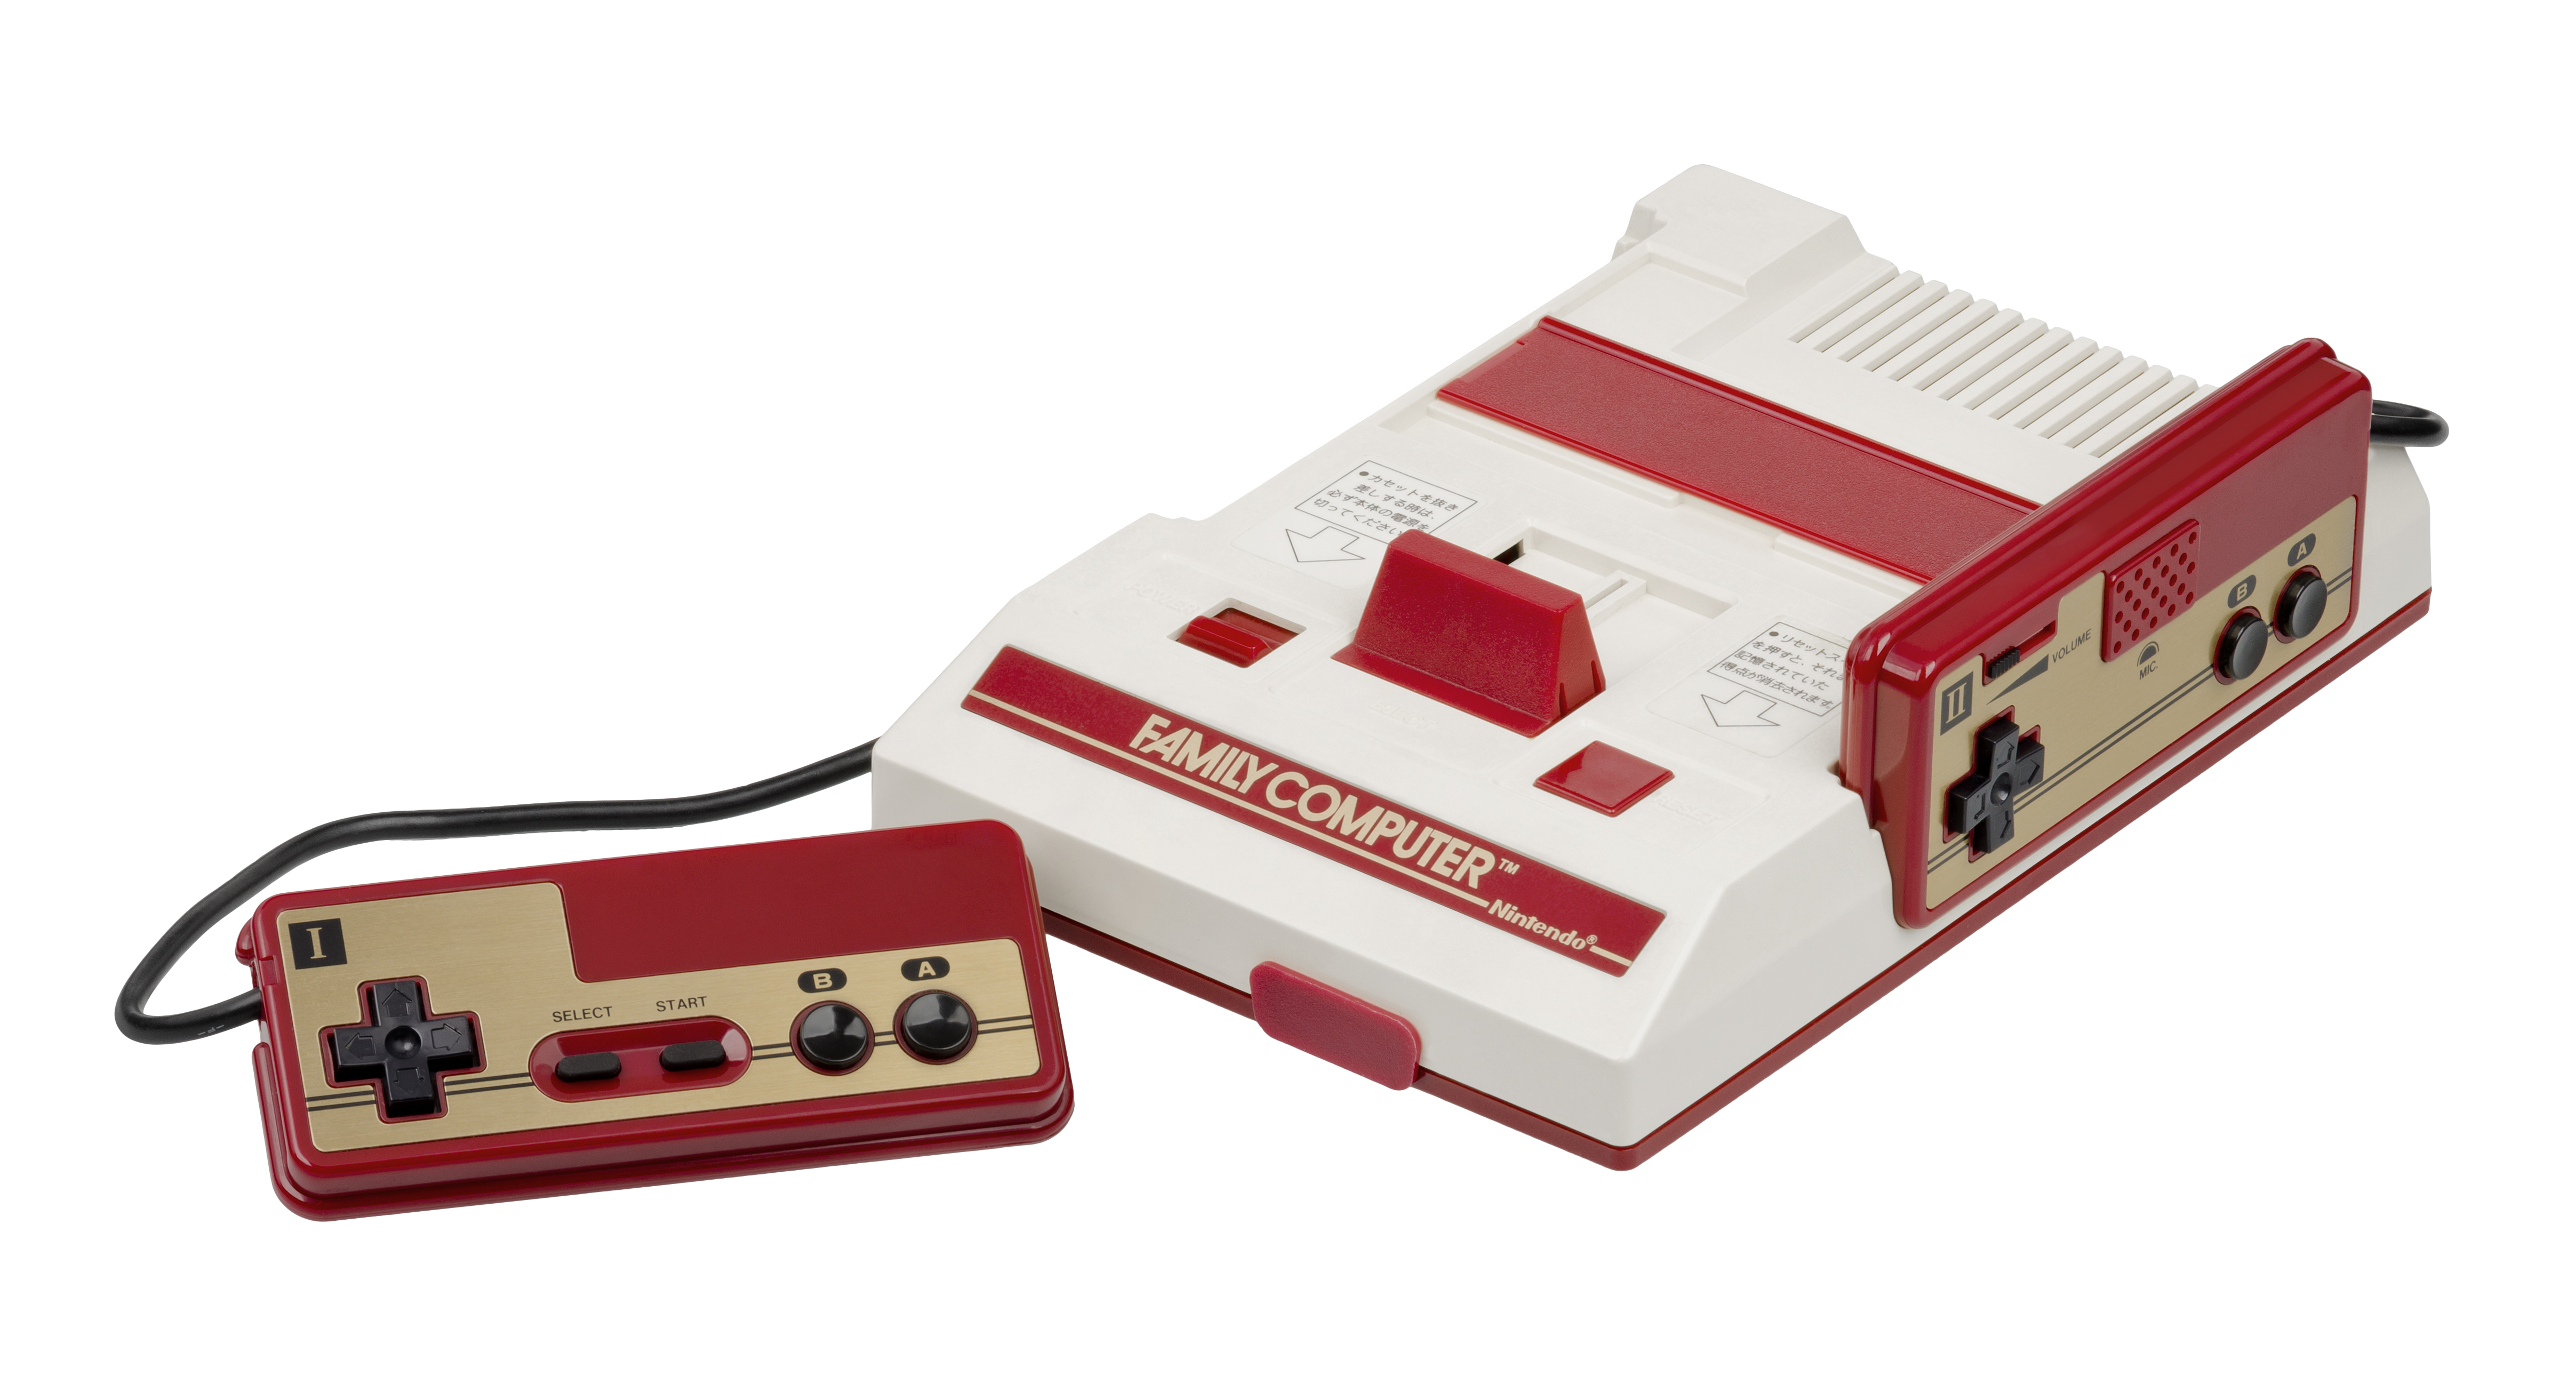
\includegraphics[width=\textwidth]{images/famicon.jpg}
		\caption{Famicon}
		\label{fig:1}
	\end{subfigure}
	%
	\begin{subfigure}[b]{0.4\textwidth}
		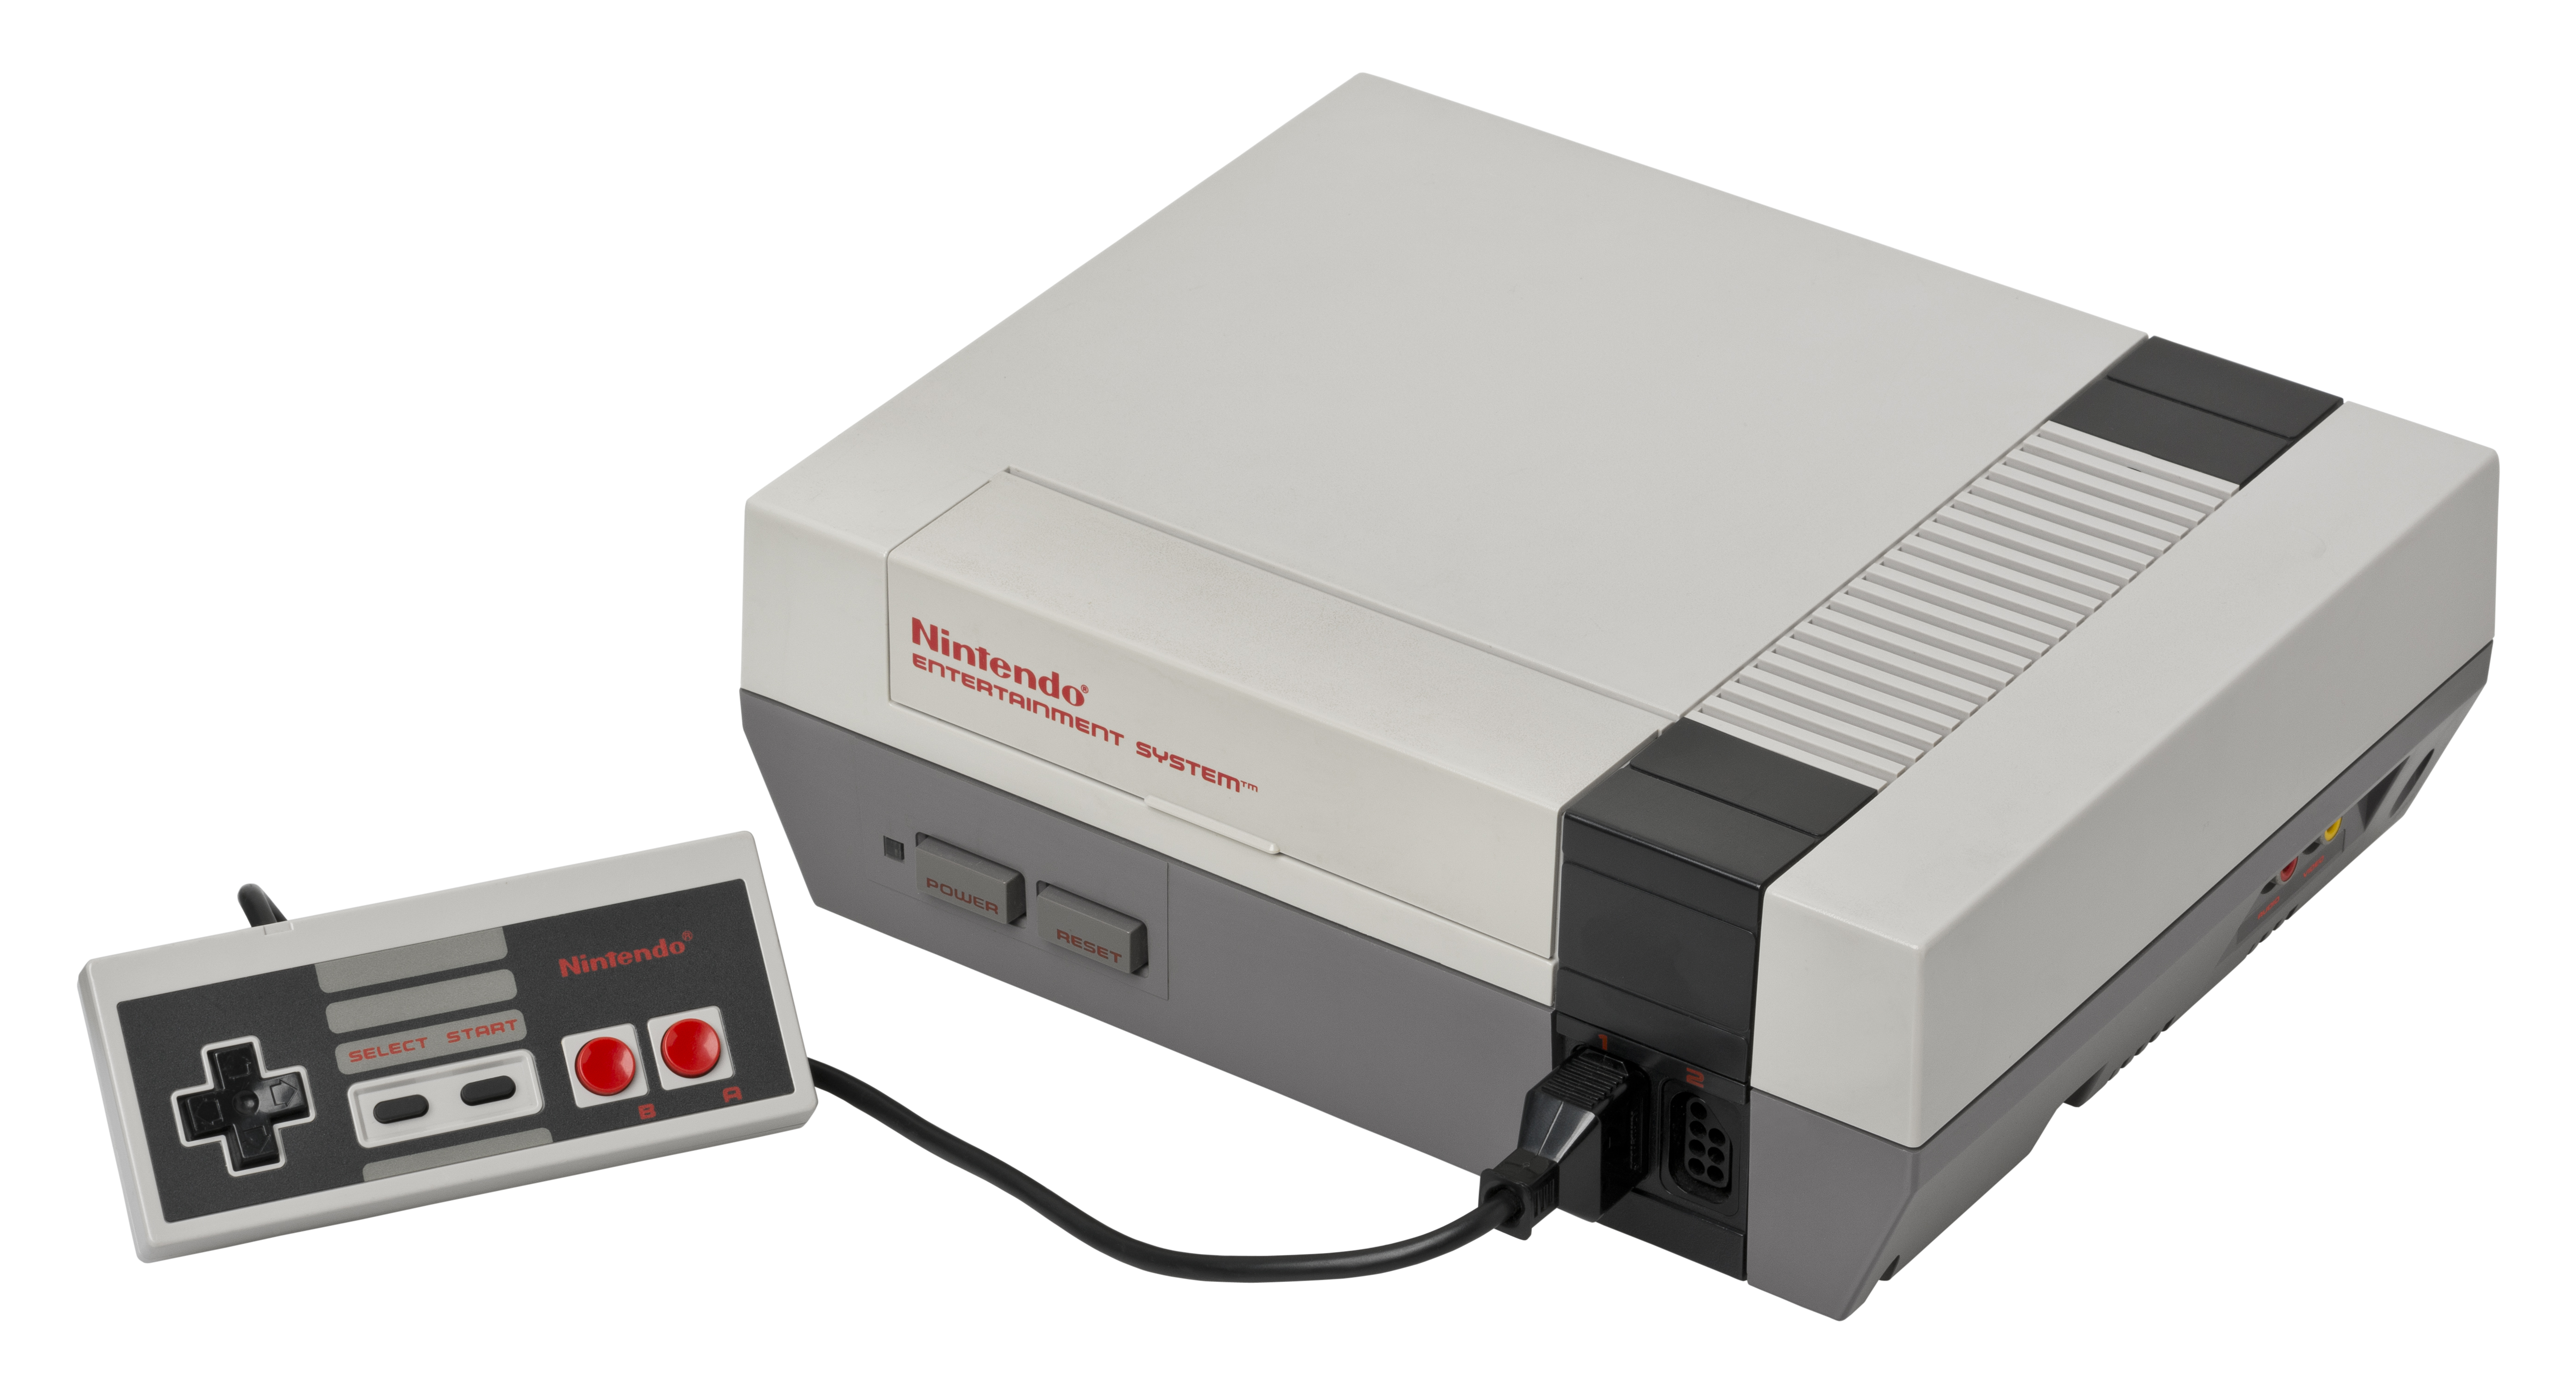
\includegraphics[width=\textwidth]{images/nes.jpg}
		\caption{NES}
		\label{fig:2}
	\end{subfigure}
	\caption{\label{fig:my-label} The console design}
\end{figure}



\section{Background}
\paragraph{ }
The NES hardware itself can be divided up to five big different part. 
\paragraph{ }
The console main chip was manufactured by Richo, which contains the CPU (Central Processing Unit) and the APU (Audio Processing Unit) (\cite{CPU}).  
The processor itself is an 8-bit MOS Technology 6502 with a little difference that the decimal mode is not presented. 
\paragraph{ }
The PPU (Pixel Processing Unit), which was also shipped by Richo, is technically a primitive graphics card which is used by the system to colour and render the graphics pixel by pixel to the Television screens.
\paragraph{ }
The Cartrdige which meant to provide the necessary binary code of the games and also the graphics data for the system. Also gave an opportunity to the developers to implement their own cartridge builds and use it to extend the console's capabilities one great example for that is the first The Legend of Zelda game. The game's cartridge also contains a battery powered RAM extension for players to save their game state (\cite{ZELD}).
\paragraph{ }
Two 8 button, these buttons are up, down, left, right, select, start, A, B, controller provided the interface for user input to the system. The NES controller was the first controller which introduced the single button plus symbol shaped DPAD. Each Nintendo system was brought some revolutionary design idea to the world of gaming console controllers.
\paragraph{ }
The RAM (Random Access Memory) is the central piece of the hardware which not only holds data but trough memory mapping it also connects all the other pieces to the CPU. Therefore the developers can control the full hardware behaviours trough with specific read and write operations to certain memory slots.
\paragraph{ }
In this project, these core parts of the hardware will be emulated on x86-64 machines. As a result, provide an application which is able to run those games which were developed for the original NES system.

\begin{figure}[!htb]
	\center{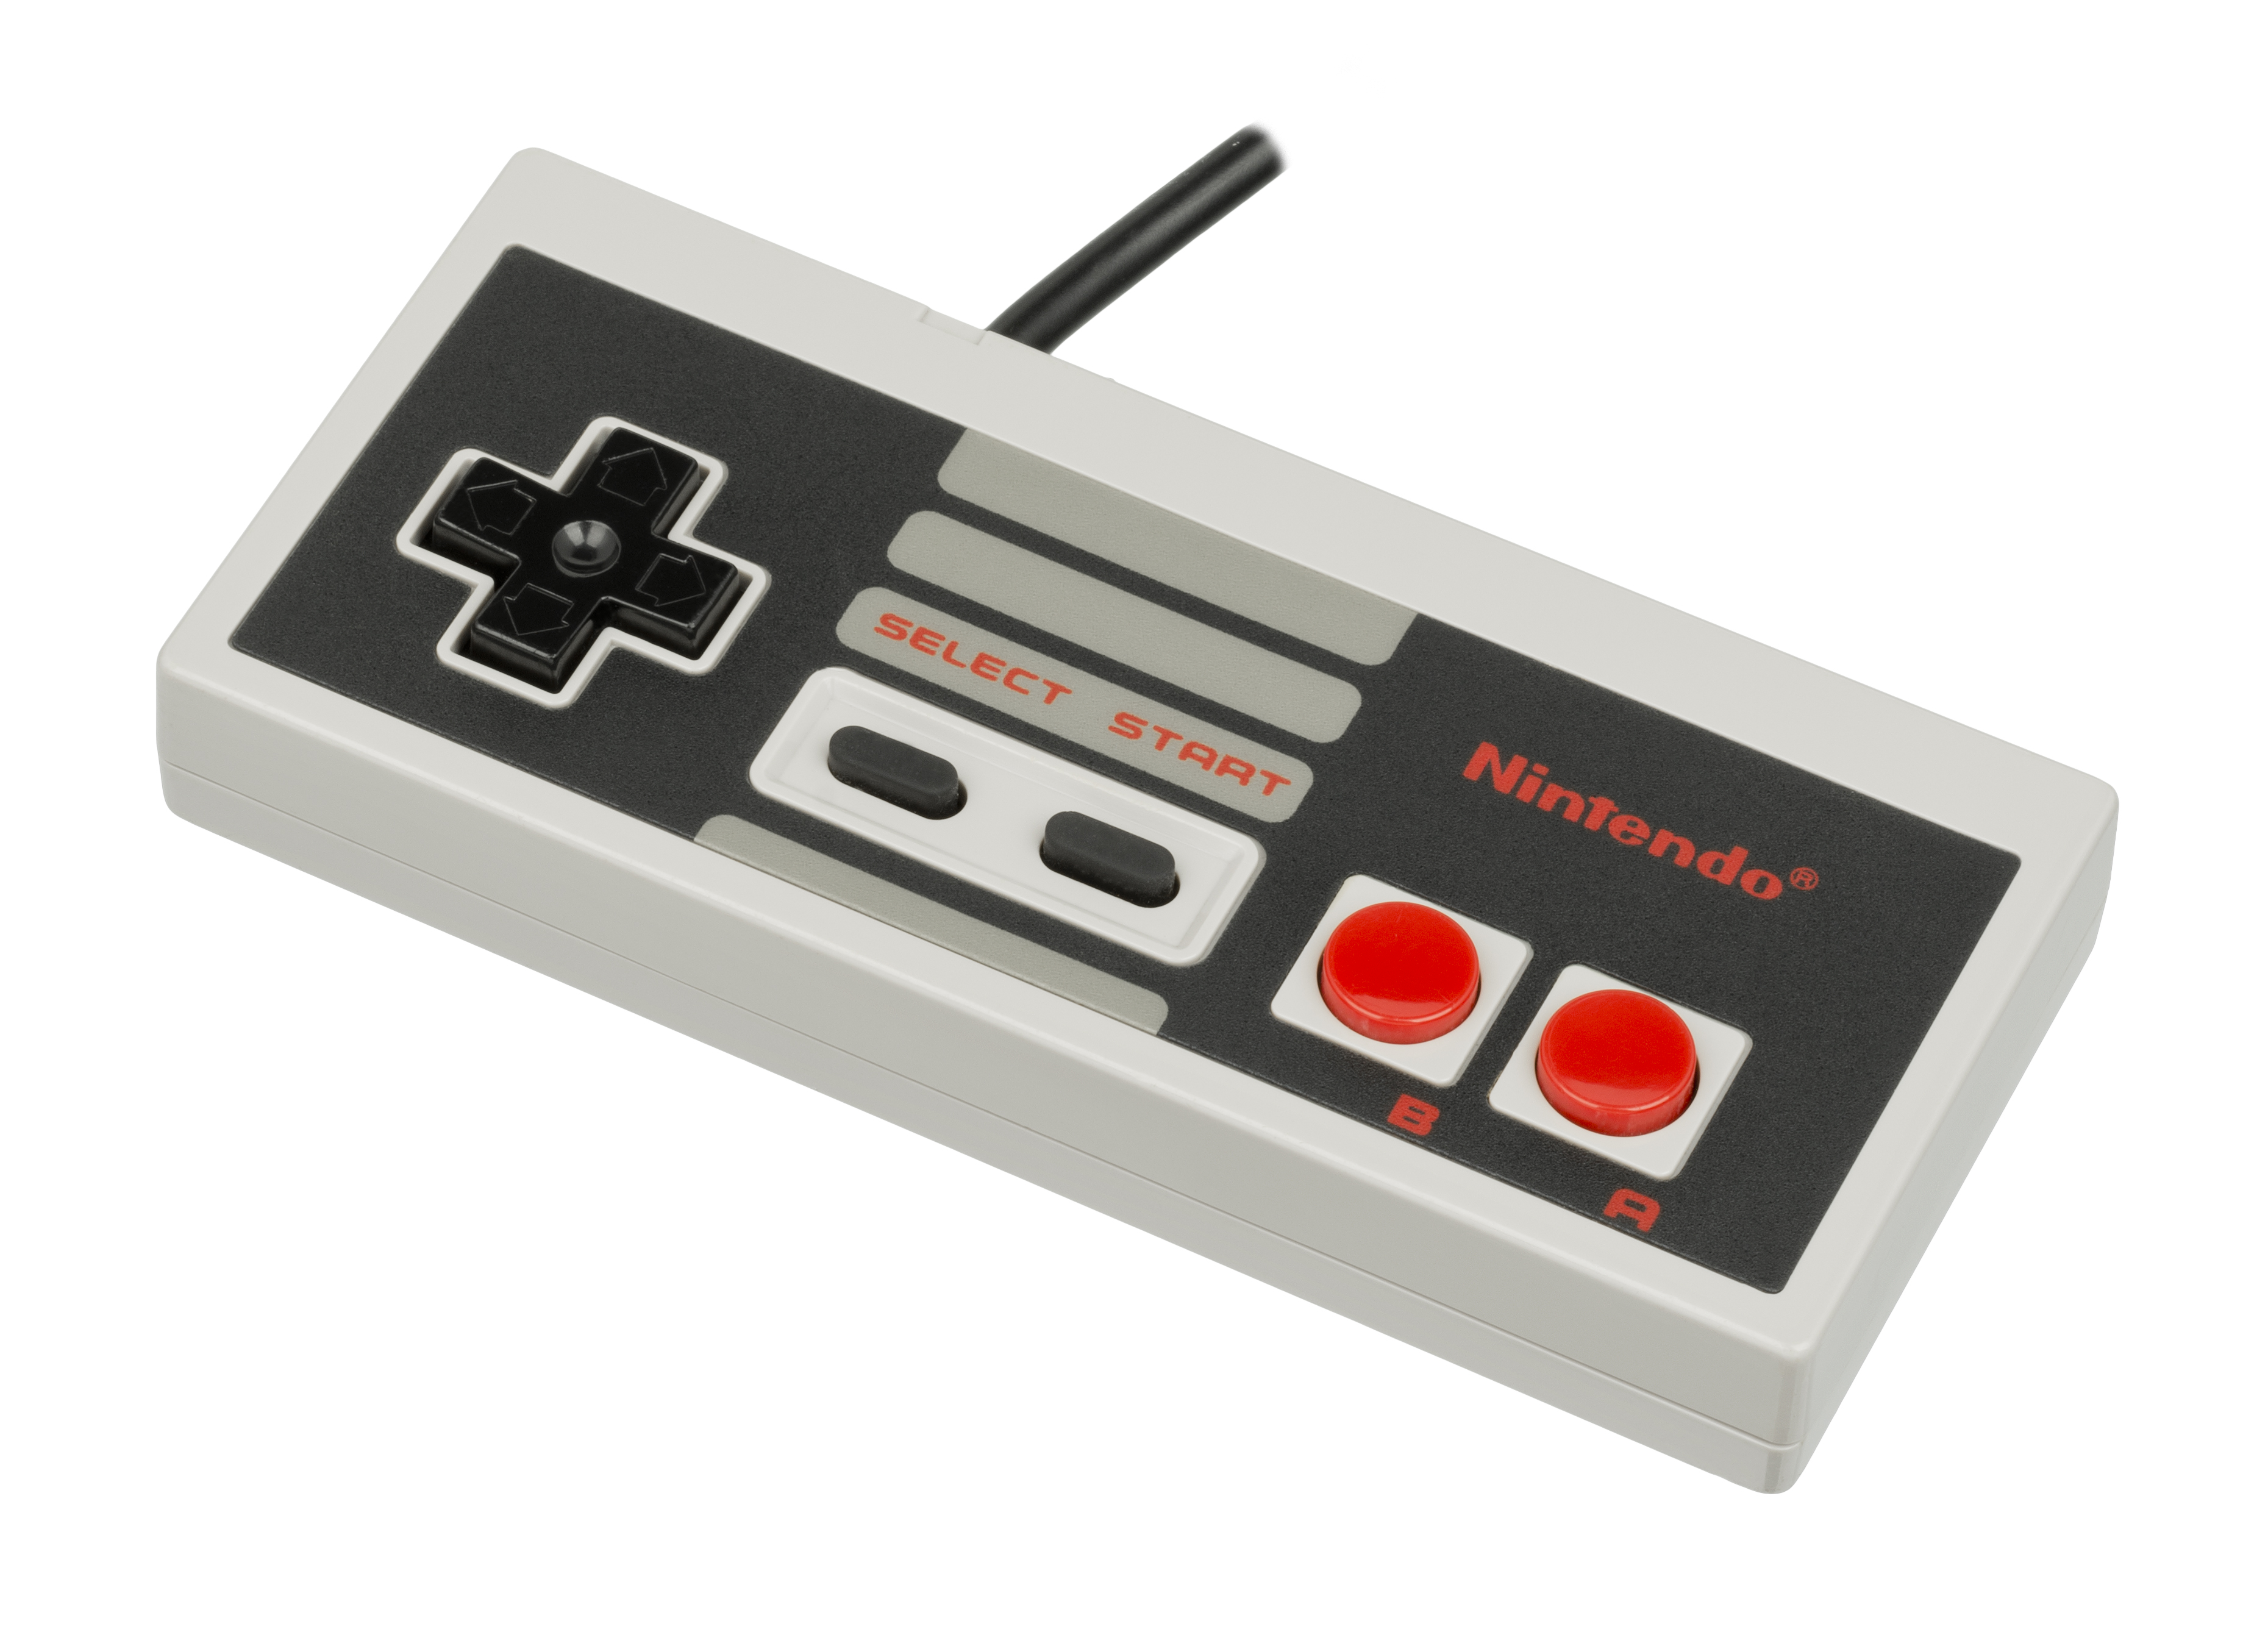
\includegraphics[width=\textwidth]
		{images/nes-controller.jpg}}
	\caption{\label{fig:my-label} NES controller}
\end{figure}



\chapter{Project Goal}
\paragraph{ }
The main target of the project is to build an application which is able to run games developed for the original Nintendo Entertainment System. The main target platform for the emulator to support is 64bit Linux, but the project design allows easy implementation for other platforms too. This goal is achieved by emulating all the necessary hardware of the original NES system programmatically thus creating a medium for the game binaries to run without any modification at all to it. 
\\ 
However, as the sounds system (APU) is not necessary to be able to run the games this part of the system is not implemented.
\\
The project goal can be divided into multiple stages which are the core and other advanced stages.
The main goal is to achieve the Minimal Core stage by the project deadline. However, if the time allows it advanced features will be implemented. 
\paragraph{Core - Minimal}
The emulator can emulate the perfectly the RAM and it's mirroring mapping behaviour properly. 
\\
The CPU capable to execute all the official operation codes, as the MOS 6502 has unofficial operation codes as well, also able to properly handle interrupts. 
\\ 
Graphics displayed on the screen with the usage of the PPU without any restriction about how it is doing it.
\\ 
The user is capable to interact with the system with a keyboard.
\\ 
Digitalized cartridge format (iNes) red and mapped with the basic NROM mapper (Mapper 0).
\paragraph{Core - Full)}
The graphics CPU and the whole system itself running with 100\% cycle accuracy compared to the original gaming console.
Some games are heavily rely on cycle accuracy, especially to provide some nice graphics implementations and also to provide more authentic experience for end users.

\paragraph{Advanced - Mappers}
Implementing additional Cartridge mappers other than the basic NROM mapper\cite{MPPR}. This would allow the emulator to run a larger pool of games.

\paragraph{Advanced - Multiple Platform}
Due to the nature of the project design, see below, support for other systems could be more easily implemented due to the modular approach which was used to develop the emulator. Therefore for instance Windows and Android could be easily supported by the emulator which would further boost the user experience.

\paragraph{Advanced - State Save}
Allowing the user to make a snapshot of the current CPU PPU and RAM state and be able to load it back at later point in case if the user would like to continue the game right from the place where they saved it.

\paragraph{Advanced - Online Multiplayer}
The NES system supports two-player local multiplayer, as the system provides hardware to connect two controllers, by default which could be extended over a network, therefore, players could play two player games with the comfort of their homes.

\chapter{Project Execution}

\section{Design}

\paragraph{ }
Due to the fact that the NES gaming console's hardware could easily be divided up to 6 distinct, loosely coupled module, it was clear that the best way is to design the implementation around these modules:
\begin{enumerate}
	\item Ram
	\item CPU
	\item PPU
	\item Controller
	\item Cartridge / Mapper
	\item APU
\end{enumerate}

This thanks to the fact that the system gives control over all of these pieces by wiring them into given memory slots and using CPU instructions to perform read and write instructions on them to trigger given actions on them, all of this without letting the actual CPU Hardware know that it is accessing anything else. Therefore when the system could be implemented module by module in careful order. Due to this modular separations, it was easy and straightforward to build each module easily by separating them up to smaller task and gradually build each module.
\paragraph{ }
Besides the separation of the emulator code to modules, the GUI, Graphical User Interface,  is also separated from the actual emulator logic. This behaviour is implemented by compiling the NES emulator logic into a shared object, dynamic library for Windows users, and linked it with the GUI implementation. This decoupling has numerous advantages over shipping the whole application as a single executable.
\\ 
Due to this separation, the emulator logic became easier to test on its own. 
\\ 
When a new patch is ready for the applications only part of the project needs to be recompiled and updated. Which makes easier to implement a versioning and updating system.
\\ 
The GUI implementation can be changed without affecting any of the core solutions therefore it is easier to port it to different platforms and devices.

\section{Tools}
\paragraph{ }
The project is written in the latest standard of C++ 17 (\cite{CPPV}). The reason behind the choice of C++ was that the language itself really stable and mature and proven to be a great tool to develop clean, stable, high performant software solutions and also providing low-level solutions for given sets of problems such as pointers. Compared to C, a system level programming language, C++ provides a more readable code on exchange for minimal performance loss thanks to it's rich standard library and object oriented programming capabilities.

\paragraph{ }
On the top of C++ a small number, namely two, of external libraries were used to develop the project.
Catch2 (\cite{CTCH}) was used to carry out the automated tests which were written for the project in a BDD (\cite{BDDT}) style.
The other one is SDL (\cite{SDL2})

\paragraph{ }
For source code compiling the GCC (\cite{GCCV}) version 8.2.1 toolchain is used through the MAKE (\cite{MAKE}) build system. And these are configured with CMake (\cite{CMKE}) to which provides a cross-platform build tool configuring interface. Also, it provides an opportunity for developers to use their own preferred IDE, Integrated Development Environment, therefore boost their productivity.

\paragraph{ }
The project documentation consists of two parts the report itself (this document) and the API doc (\cite{APID}).
\\
The report was created with LaTeX (\cite{LATX}). On the other hand, the API documentation was generated with Doxygen (\cite{DOXY}) from the annotated C++ Header files of the source code.

\paragraph{ }
The source code along with the build system configuration and the documentation is version controlled with GIT and stored in a main  Github repository (\cite{REPO}).
As the project meant to be published as an open source project it is publicly available. Although, under the time of the project during the course of the project it was also publicly available the repository was strictly available for editing for the project owner (Sebestyén Bence) and the project supervisor (Robert Atkey).
\\
The project repository is also linked to a CI, Continuous Integration, the system called Travis CI (\cite{TRAV}). Which mostly used to provide security against merging any proposed changes which are not passing the build state or failing any of the automated tests which were supplied with the source code. The CI system build and testing are triggered every time when a pull request for a change against the main repository is set up and blocking any merge until the errors within the proposed changes are not fixed.



\section{Management}

\paragraph{ }
The development cycle managed through GitHub project page. For every task regarding the project execution, there was an issue opened. These issues were labelled up based on which development cycle, see below, it was accomplished, and added to the given project milestone based on which module it was belonged to.
\\
This provided a great oversight over the project's evolution and also a faster more stable development cycle due to the small subtasks.

\paragraph{ }
The development life cycle contains multiple stages which are built upon each other. These life cycle stages are the following:

\begin{enumerate}
	\item Planing
	\item Prototyping
	\item Implementing
	\item Testing
	\item Documenting
\end{enumerate}

\paragraph{ }
Every small task went through a planning phase which mostly consisted idea how to actually code down the given task and how it is going to be fitting into the whole project current state meanwhile thinking about to keep as much space as possible for later new features and improvements.

\paragraph{ }
Prototyping itself was kinda more flexible, compared to the planning, it was different from task to task, some sort of prototype was also developed outside the project source to prove concepts of the planning, but the difference was that it was not always done to every single subtask. Sometimes it involved a whole module, sometimes it just has done for two tasks together.
\\
The main goal here was to test the result of the planning in an actual working context and see if the result is clean, stable and extendable enough to be implemented in the actual project.

\paragraph{ }
Through the implementation, the actual result of the planning and prototyping were added to the main code base.

\paragraph{ }
Testing was carried out in two phases. Depending on the given issue, manual testing was carried out on task and a subtask level if it was needed and also automated BDT, Behaviour Driven Testing, where implemented for every module to test their provided functionality. And these automated tests were executed with the CI as well.

\paragraph{ }
The API documentation were created after the given task was finished and updated with Doxygen.
\\
Meanwhile, the report itself was uprated in larger chunks because this way there was always a bigger portion of the system was available therefore it was easier to position the actual chunk to the whole project.

\begin{figure}[!htb]
\center{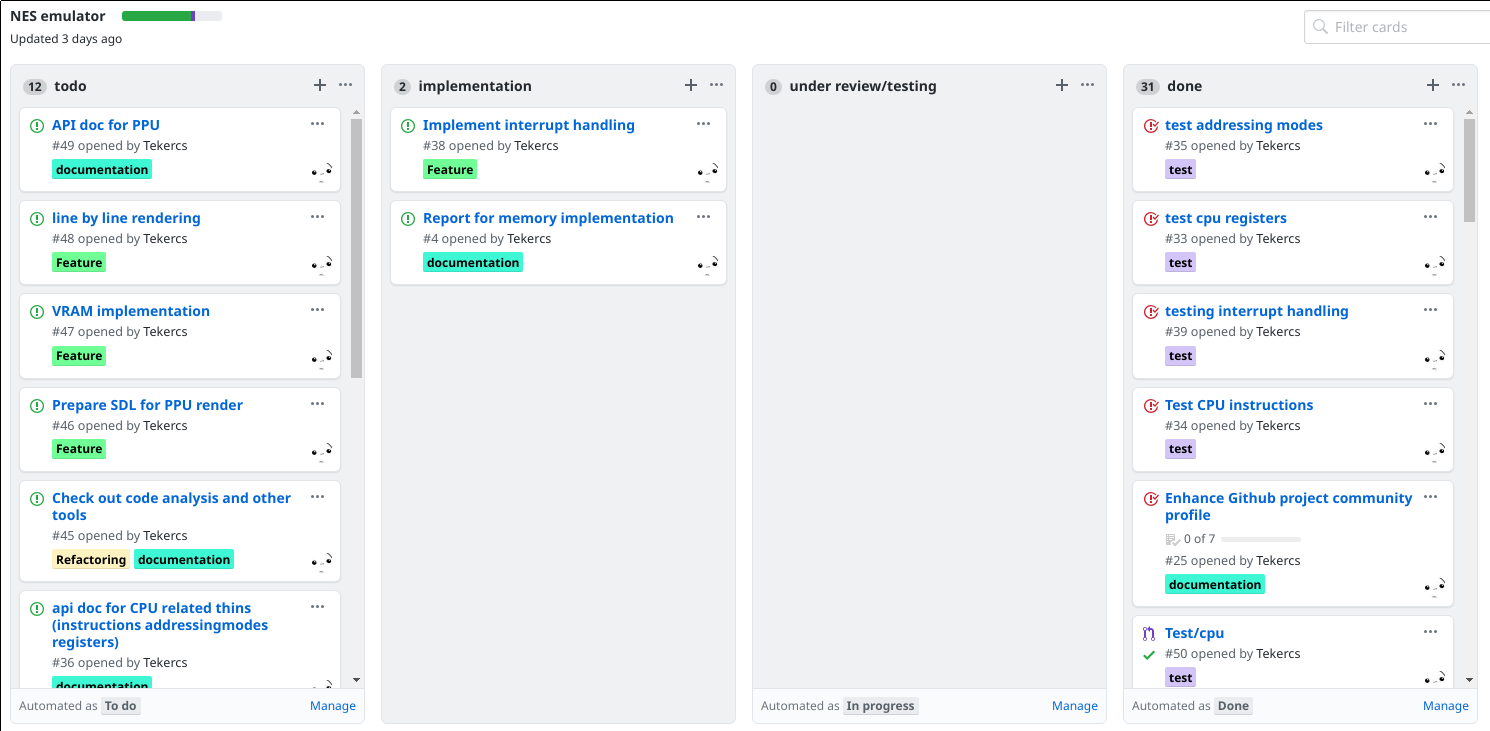
\includegraphics[width=\textwidth]
	{images/github_project.png}}
\caption{\label{fig:my-label} Github project page}
\end{figure}

\chapter{Specification and implementation}

\section{RAM}

\subsection{Specification}

\subsection{Implementation}

\subsection{Testing}

\section{Cartridge (ROM)}

\subsection{Specification}

\subsection{Implementation}

\subsection{Testing}

\section{CPU}

\subsection{Specification}

\subsection{Implementation}

\subsection{Testing}

\section{PPU}

\subsection{Specification}

\subsection{Implementation}

\subsection{Testing}

\chapter{Evaluation}

\section{Performance and Precision}

\section{Game Performance}

\chapter{Conclusions}

\printbibliography

\end{document}          